\documentclass[xcolor={dvipsnames}]{beamer}
\usepackage{../common/scicomp}

\title{Introduction to Parallel Programming}
\date{October 14, 2016}

\lstset{language=C++,
	basicstyle=\ttfamily,
	keywordstyle=\color{blue}\ttfamily,
	stringstyle=\color{red}\ttfamily,
	commentstyle=\color{ForestGreen}\ttfamily,
	morecomment=[l][\color{magenta}]{\#}
}

\begin{document}

\begin{frame}
	\titlepage
\end{frame}

\begin{frame}{Outline}
	\tableofcontents
\end{frame}

	
\section{The basics}

\begin{frame}[fragile]{Hello World!}{}
This code simply prints ``Hello World!''.
\begin{lstlisting}
#include <stdlib.h>
#include <stdio.h>

int main() {
   printf("Hello World!\n");
   return 0;
}
\end{lstlisting}	
\end{frame}

\subsection{Data types}
\begin{frame}[fragile]{C++ has explicit data types.}{}
\begin{lstlisting}
bool isEmpty = true;

int particles = 1024;

float Tf = 273.15;

double phi = 1.61803398875;
\end{lstlisting}	
\end{frame}

\begin{frame}[fragile]{Structs are complex data types.}{}
We can define the 3D vector data type.
\begin{lstlisting}
struct float3{
   float x, y, z;
};

float3 pos;
pos.x = 3.2;
pos.y = -4.7;
pos.z = 1.34;
\end{lstlisting}	
\end{frame}

\subsection{Pointers}
\begin{frame}{A pointer is a variable that stores \\ the memory address of another variable.}{}
\begin{itemize}[<+->]
\item When a variable is declared, the memory needed to store its value is assigned to a specific location.
\bigskip
\item The program does not explicitly decide the exact memory location.
\bigskip
\item A pointer is used to access data cells that are at a certain postion relative to it.
\end{itemize}
\end{frame}

\begin{frame}[fragile]{Pointers may be obtained from values and viceversa.}
\begin{itemize}[<+->]
\item \texttt{\&} is the address-of operator, and can be read simply as "address of"
\item \texttt{*} is the dereference operator, and can be read as "value pointed to by"
\end{itemize}

\pause
\begin{lstlisting}
float val;  \\ val is declared as a variable
float *ptr; \\ ptr is declared as a pointer

val=0.577;
*ptr=0.577;

printf("Address of val %d\n", &val);
printf("Address of *ptr %d\n", ptr);
\end{lstlisting}

\end{frame}

\begin{frame}[fragile]{An array may be declared with a pointer.}{}

\begin{lstlisting}
int N = 1024;
double *foo = new double[N];

for(int i=0; i<N; i++){
   foo[i]=cos(pi/N*i));
}
\end{lstlisting}

\pause
The pointer \texttt{foo} refers to the memory address of the first element \texttt{foo[0]}.

\pause
\bigskip
The pointer \texttt{foo+k}, where \texttt{k} is an integer, refers to the memory address of the k-th element \texttt{foo[k]}.
\end{frame}

\begin{frame}[fragile]{Matrices are square-shaped arrays.}{}



A matrix of size $m\times n$ may be indexed in column-major storage
\begin{lstlisting}
int m=128, n=256;
double *A = new double[m*n];
\end{lstlisting}
\pause
\begin{lstlisting}
for(int i=0; i<m; i++){
   for(int j=0; j<n; j++){
      A[j*m+i]=cos(pi/m*i*j);
   }
}
\end{lstlisting}
\end{frame}



\section{Parallel programming}

\begin{frame}[fragile]{Why parallelism?}{}
\begin{quote}
If you were plowing a field, which would you rather use: Two strong oxen or 1024 chickens?
\end{quote}
Seymour Cray, the father of supercomputing.

\vfill
\begin{figure}[H]
\centering
\begin{subfigure}{.4\textwidth}
	\centering
	\includegraphics[height=0.3\textheight]{oxen}
\end{subfigure}
\begin{subfigure}{.4\textwidth}
	\centering
	\includegraphics[height=0.3\textheight]{chickens}
\end{subfigure}
\label{fig:cray}
\end{figure}

\end{frame}


\begin{frame}[fragile]{Parallelization is desired to increase the throughput.}{}
Throughput = Number of computations / Amount of time.

\pause
\bigskip
Throughput is measured in \textbf{FL}oating-\textbf{P}oint \textbf{O}perations \textbf{P}er \textbf{S}econd or \textbf{flops}.
\end{frame}


\subsection{Hardware}
\begin{frame}{The CPU is excellent for serial tasks.}

\begin{itemize}[<+->]
\item The CPU is in charge of coordinating hardware and software.
\bigskip
\item Typically, it may have from 2 to 12 processing cores.
\bigskip
\item Many programs run entirely on the CPU. 
\end{itemize}

\begin{figure}
\centering
\includegraphics[height=0.3\textheight]{corei7}
\label{fig:corei7}
\end{figure}
\end{frame}

\begin{frame}{The GPU is excellent for parallel tasks.}
\begin{itemize}[<+->]
\item The GPU is in charge of processing and rendering graphics onto your display.
\bigskip
\item Typically, it may have from hundreds to thousands of processing cores.
\bigskip
\item General Purpose GPU Programming takes advantage of this enormous computing power.
\end{itemize}

\begin{figure}
\centering
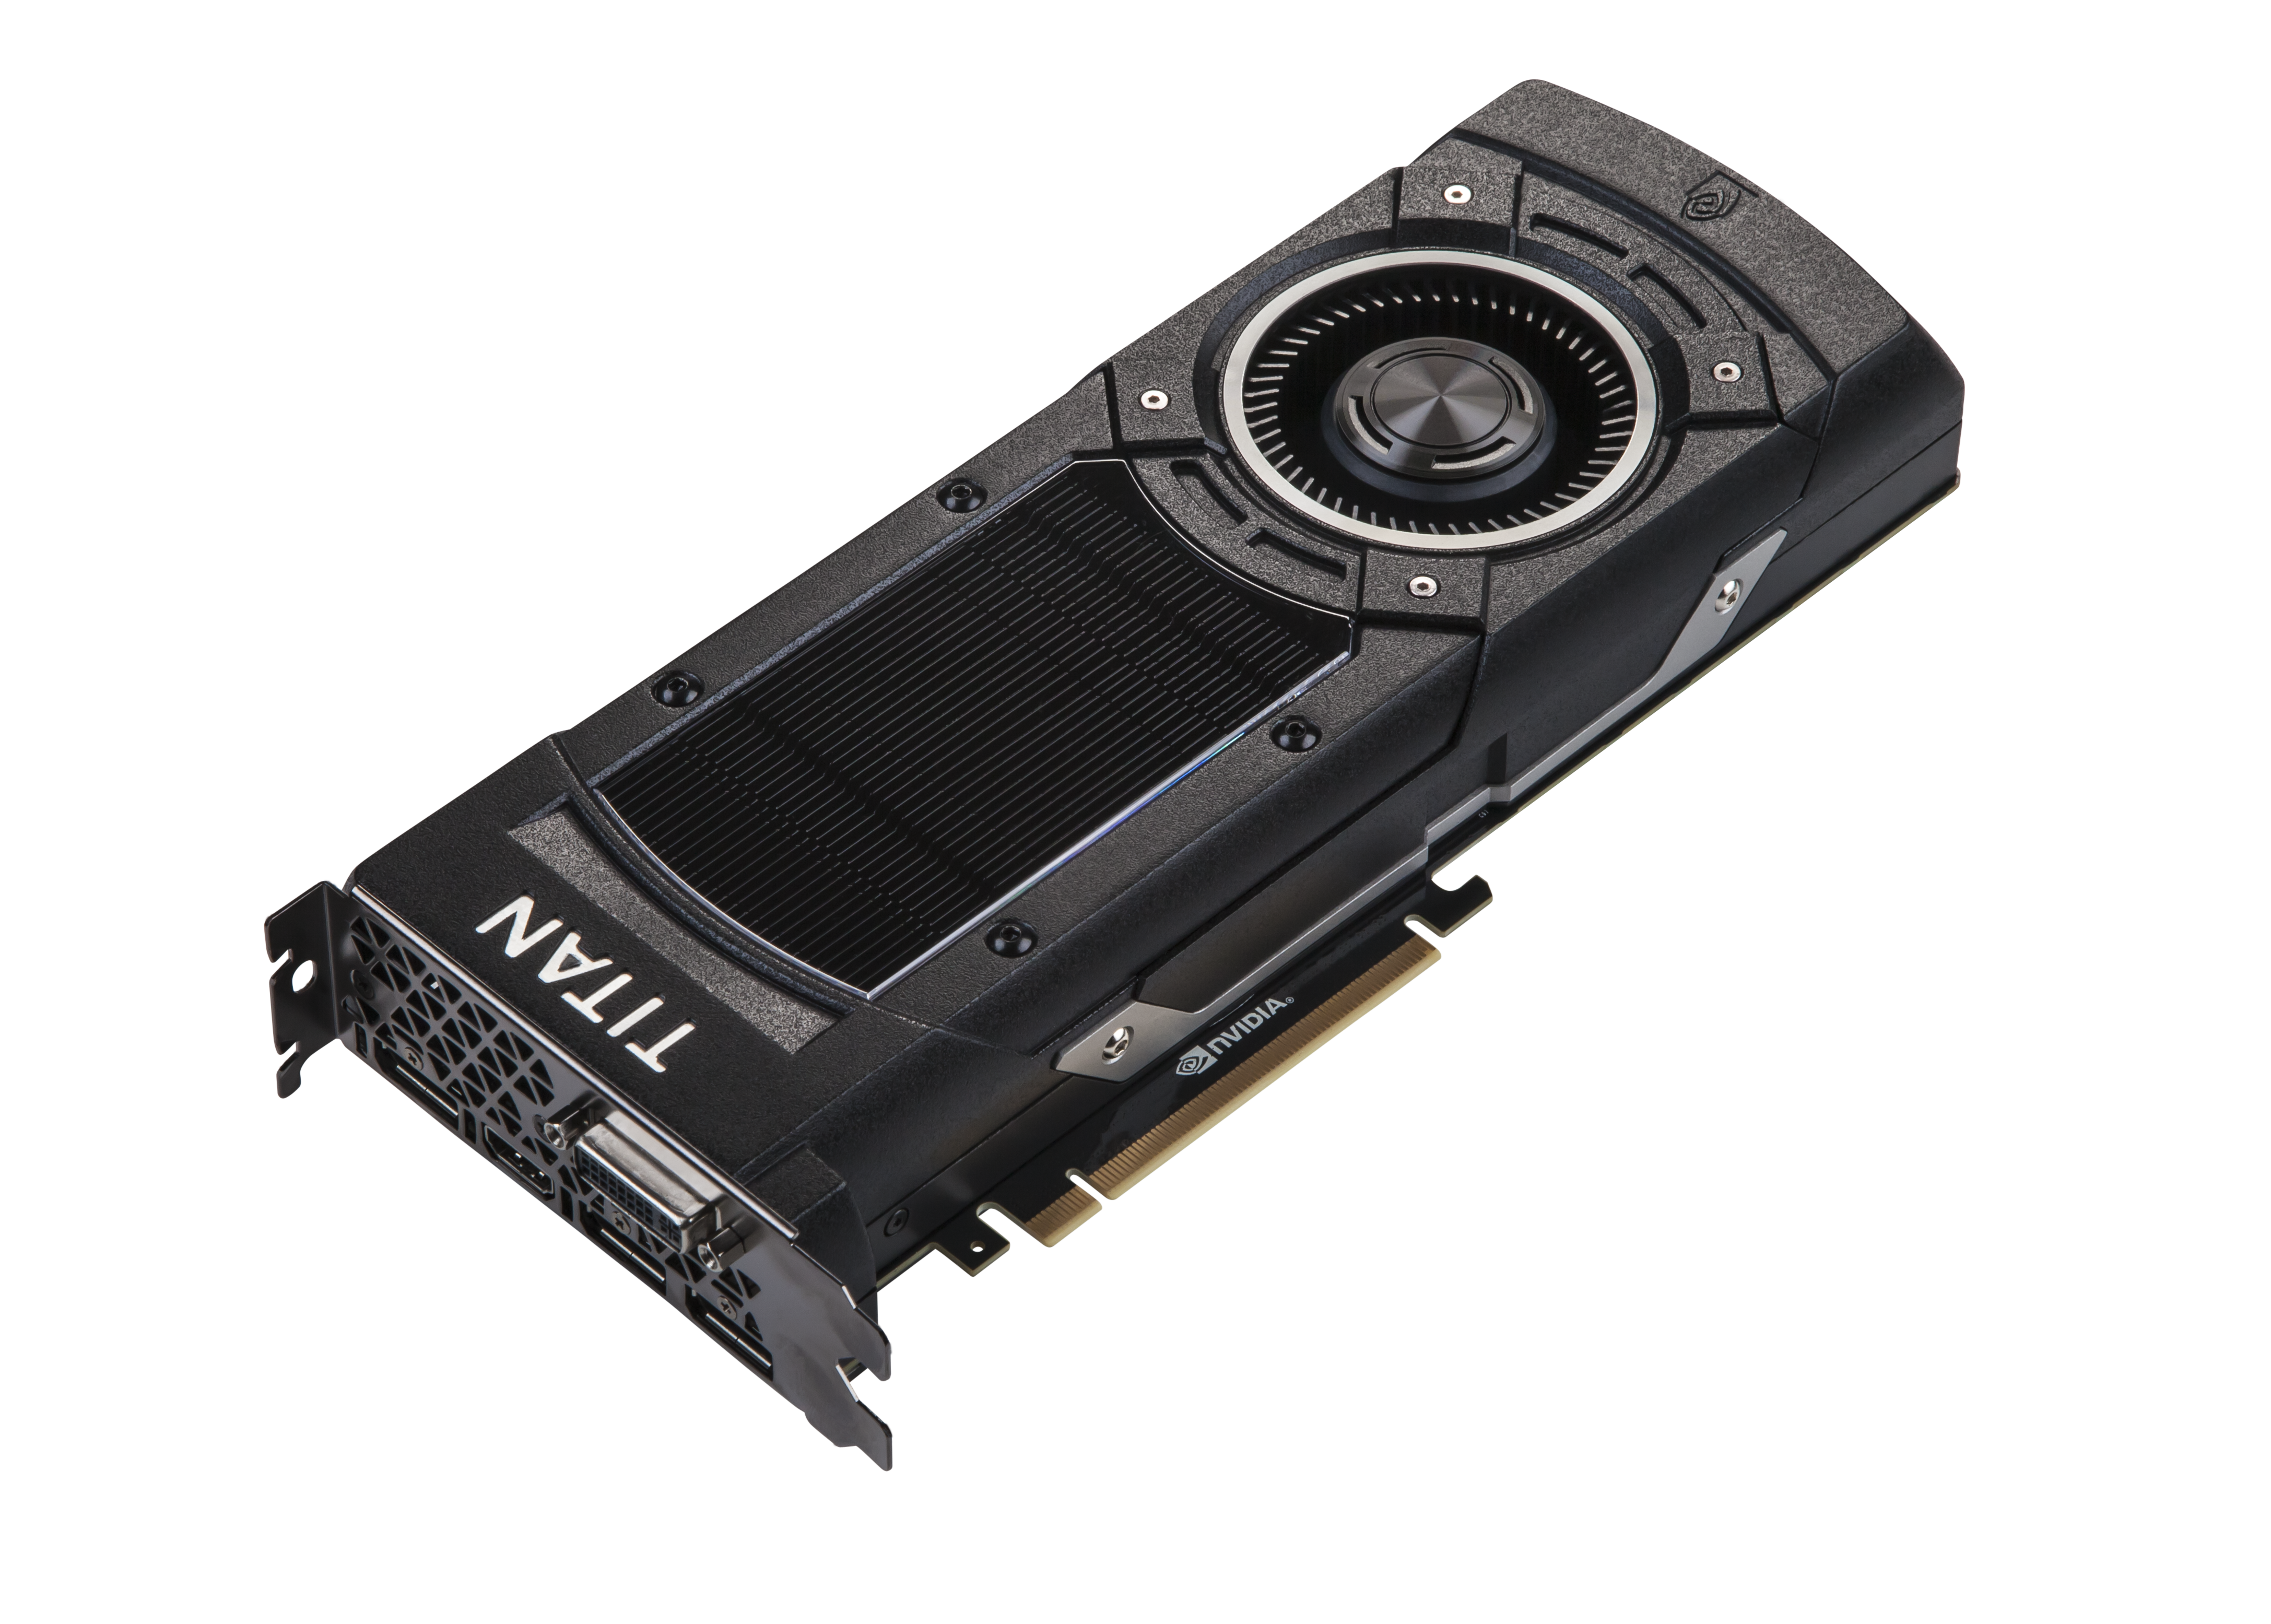
\includegraphics[height=0.3\textheight]{titan}
\label{fig:titan}
\end{figure}
\end{frame}


\begin{frame}{The GPU devotes more transistors to data processing.}
GPUs have many more Arithmetic Processing Units (ALUs).
\begin{figure}
\centering
\includegraphics[height=0.4\textheight]{cpugpu}
\label{fig:cpugpu}
\end{figure}
\end{frame}

\subsection{Parallel primitives}

\begin{frame}{Parallel primitives are common, highly parallelizable operations}{}

\begin{itemize}
\item Mapping
\item Stencil
\item Reduction
\item Scan or prefix sum
\end{itemize}
\end{frame}

\begin{frame}{Mapping}{}
A mapping is a transformation of $N$ inputs into $N$ outputs where the same \textbf{unary function} is applied \textbf{independently} to every array element.
\pause 
\begin{equation*}
y_i=f(x_i),\qquad i=0,1,\ldots,N-1.
\end{equation*}

\begin{itemize}[<+(1)->]
\item Compute the square of each array element.
\item Compute the color of each pixel on an image.
\item Transform each vertex of a 3D model.
\end{itemize}
\end{frame}

\begin{frame}{Stencil}{}
A stencil operation is a transformation of $N$ inputs into $N$ outputs where the operator takes some of the neighboring elements.
\pause 
\begin{equation*}
y_i=f(\ldots,x_{i-1},x_i,x_{i+1},\ldots),\qquad i=0,1,\ldots,N-1.
\end{equation*}

\begin{itemize}[<+(1)->]
\item Finite differences.
\item Image filtering.
\item Convolutional Neural Networks.
\end{itemize}
\end{frame}

\begin{frame}{Reduction}{}
A reduction operation takes $N$ inputs to produce a single output with an \textbf{associative binary operator}.
\pause 
\begin{equation*}
y=x_0 \oplus x_1 \oplus ... \oplus x_{N-1}
\end{equation*}

\begin{itemize}[<+(1)->]
\item Find the total sum of an array.
\item Find the maximum element of an array.
\item Find the minimum element of an array.
\end{itemize}
\end{frame}

\begin{frame}{Scan or prefix sum}{}
A scan operation takes $N$ inputs to produce $N$ partial outputs by applying an \textbf{associative binary operator}.
\pause 
\begin{equation*}
y_i=x_0 \oplus x_1 \oplus ... \oplus x_{i}, \qquad i=0,1,\ldots,N-1
\end{equation*}

\begin{itemize}[<+(1)->]
\item Find the accumulated sum of an array.
\item Compute the histogram of a series of data.
\item Image processing, High Dynamic Range (HDR).
\end{itemize}
\end{frame}

\begin{frame}{Parallel primitives are already\\ implemented on libraries}{}

Thrust is a CUDA library that allows you to implement high performance parallel applications with minimal programming effort.

\vfill
\begin{figure}
\centering
\includegraphics[height=0.25\textheight]{thrust}
\label{fig:thrust}
\end{figure}
\end{frame}


\section{The CUDA programming model}

\subsection{Thread Hierarchy}
\begin{frame}{Parallel code execution is organized into\\ a grid of thread blocks.}
\begin{figure}
\centering
\includegraphics[width=0.7\linewidth]{threads}
\label{fig:threads}
\end{figure}
\end{frame}

\begin{frame}{Various threads execute serial code simultaneously.}
\begin{itemize}[<+->]
\item These pieces of serial code are known as \textbf{kernels}.
\bigskip
\item Their execution is grouped into \textbf{thread blocks}.
\bigskip
\item Thread blocks are grouped into a \textbf{block grid}.
\bigskip
\item Threads and blocks may have up to three-dimensional indices.
\end{itemize}
\end{frame}

\begin{frame}{Parallelism is limited by the GPU.}
Since the whole task might require more parallel processors that the ones that are available, the task is divided into thread blocks.

\pause
\bigskip
All threads within a thread block are ensured to be synchronous.
\end{frame}

\subsection{Memory Hierarchy}

\begin{frame}{Memory is shared at different levels.}
\begin{figure}
\centering
\includegraphics[width=0.5\linewidth]{memory}
\label{fig:memory}
\end{figure}
\end{frame}

\begin{frame}{Memory is shared at different levels.}
\begin{itemize}[<+->]
\item \textbf{Local memory} is the fastest, but it is limited to an individual thread.

\bigskip
\item \textbf{Shared memory} is shared between threads of the same block.

\bigskip
\item \textbf{Global memory} is the slowest, but may be accessed from any thread.
\end{itemize}
\end{frame}

\subsection{Simple code example}
\begin{frame}[fragile]{Memory allocation. Oh, no! pointers!}
The CUDA unified memory model allows sharing between the host and the device. This is how to allocate global memory on the device.

\begin{lstlisting}
int N=1024;
float *data;
cudaMallocManaged(&data, N*sizeof(float));
\end{lstlisting}
\end{frame}

\begin{frame}[fragile]{Kernel declaration. Oh, no! weird syntax!}
\begin{lstlisting}
// Generate equally spaced vector from a to b

__global__ void linspace(int N, float *data,
                         float a, float b){
   int i=blockIdx.x*blockDim.x+threadIdx.x;
   data[i]=a+(b-a)*i/(N-1);
}
\end{lstlisting}
\pause
\begin{lstlisting}
// Compute the square of each array element

__global__ void mapsquare(int N, float *data){
   int i=blockIdx.x*blockDim.x+threadIdx.x;
   data[i]=data[i]*data[i];
}
\end{lstlisting}	
\end{frame}

\begin{frame}[fragile]{Kernel invocation. Oh, no! even weirder syntax!}
\begin{lstlisting}
// Define grid and block dimensions
dim3 block(512);
dim3 grid((N+512-1)/512);

// Kernel invocation
linspace<<<grid, block>>>(N, data, -10, 10);

mapsquare<<<grid, block>>>(N, data);
\end{lstlisting}
\end{frame}

\begin{frame}[fragile]{We forgot our data on the device,\\ we must take it back to the host.}
\begin{lstlisting}
// Must do this before passing data
// from device to host
cudaDeviceSynchronize();

// Print the result
for(int i=0; i<N; i++){
   printf("%f\n", data[i]);
}
\end{lstlisting}
\end{frame}

\begin{frame}{Conclusion}
Efficient parallel programming may seem very complicated at first, but its benefits are truly worth the effort.

\pause
\bigskip
If you really liked it, enroll to the Introduction to Parallel Programming Course on Udacity.
\end{frame}


\begin{frame}{References}
\nocite{*}
\bibliographystyle{ieeetr}
\bibliography{references.bib}
\end{frame}
	
\end{document}